\section{ODE Simplification}
% TODO: Add ODE Simplfication Examples
A primary application of Fourier Analysis is to simplify higher-order ODE systems into lower-order ODE systems. This can greatly reduce the complexity of the problem and can allow for either simpler analytical solutions or numerical solutions using Euler's Method or Runge-Kutta methods. The following examples aim to illustrate this application of Fourier Analysis \citep{Libretexts_2021b}.

\subsection{Driven Simple Harmonic Oscillator with Damping}
The following ODE for a Driven Simple Harmonic Oscillator with Damping represents the dynamic equation governing the motion of a mass subjected to both a restoring force and an external driving force while dissipating energy due to damping.

\subsubsection{Definition}
Let us define a Simple Harmonic Oscillator (SHO) of mass \(m\) and is attached to a spring with spring constant \(k\).
The SHO is subject to a damping force with damping coefficient \(\gamma\) and an additional driving force \(f(t)\).

\vspace{5mm}

Define \(\omega_0 = \sqrt{\frac{k}{m}}\) as the natural frequency of the SHO and the damping force as \(F_d = -2 m \gamma v\), where \(v\) is the velocity of the SHO.

\noindent
Using Newton's Second Law,
\begin{align}
    \Sigma F = ma &= -m \omega_0^2 x - 2 m \gamma v + f(t) \\
    m \frac{d^2 x}{dt^2} &= -m \omega_0^2 x - 2 m \gamma \frac{dx}{dt} + f(t)
\end{align}

\noindent
Dividing by \(m\) and rearranging terms, we get the following differential equation for a driven SHO with damping \citep{Libretexts_2021a}:

\begin{equation} \label{eq:driven_sho_equation}
    \frac{d^2 x}{dt^2} + 2 \gamma \frac{dx}{dt} + \omega_0^2 x(t) = \frac{f(t)}{m}
\end{equation}

\subsubsection{Application of the Fourier Transform}
\noindent
Let us take the Fourier Transform of \cref{eq:driven_sho_equation} with respect to \(t\). Thus, let \(X(\omega)\) and \(F(\omega)\) be the respective Fourier Transforms of \(x(t)\) and \(f(t)\) with respect to \(t\).

\begin{equation}
    \mathcal{F}_t \left\{ \frac{d^2 x}{dt^2} + 2 \gamma \frac{dx}{dt} + \omega_0^2 x(t) \right\} = \mathcal{F}_t \left\{ \frac{f(t)}{m} \right\}
\end{equation}

\noindent
Using \cref{fourier_linearity},
\begin{equation} 
    \mathcal{F}_t \left\{ \frac{d^2 x}{dt^2} \right\} + \mathcal{F}_t \left\{ 2 \gamma \frac{dx}{dt} \right\} + \mathcal{F}_t \left\{ \omega_0^2 x(t) \right\} = \mathcal{F}_t \left\{ \frac{f(t)}{m} \right\}
\end{equation}

\noindent
Using \cref{fourier_scaling},
\begin{equation} 
    \mathcal{F}_t \left\{ \frac{d^2 x}{dt^2} \right\} + 2 \gamma \mathcal{F}_t \left\{ \frac{dx}{dt} \right\} + \omega_0^2 \mathcal{F}_t \left\{ x(t) \right\} = \frac{\mathcal{F}_t \left\{ f(t) \right\}}{m} 
\end{equation}

\noindent
Using \cref{fourier_derivative},
\begin{align}
    \mathcal{F}_t \left\{ \frac{dx}{dt} \right\} &= i \omega \mathcal{F}_t \left\{ x(t) \right\} \\
    &= i \omega X(\omega) + C_1 \\
    \mathcal{F}_t \left\{ \frac{d^2 x}{d t^2} \right\} & = i \omega \mathcal{F}_t \left\{ \frac{dx}{dt} \right\} \\
    & = -\omega^2 X(\omega) + i \omega C_1 + C_2
\end{align}

\noindent
Therefore,
\begin{align}
    -\omega^2 X(\omega) + i \omega C_1 + C_2 + 2 \gamma i \omega X(\omega) + 2 \gamma C_1 + \omega_0^2 X(\omega) = \frac{F(\omega)}{m} \\
    X(\omega) \left( \omega_0^2 - \omega^2 + 2 \gamma i \omega \right) = \frac{F(\omega) - m C_1 \left( i \omega + 2 \gamma \right) - m C_2}{m}
\end{align}

\noindent
Thus,
\begin{equation} \label{eq:driven_sho_fourier}
    X(\omega) = \frac{F(\omega) - m C_1 \left( i \omega + 2 \gamma \right) - m C_2}{m \left( \omega_0^2 - \omega^2 + 2 \gamma i \omega \right)}
\end{equation}

By applying the Fourier Transform to the driven SHO equation, we have reduced the problem from solving a second order ODE (\cref{eq:driven_sho_equation}) to solving a simple algebraic equation (\cref{eq:driven_sho_fourier}). This is a significant reduction in complexity.

Once we have solved for \(X(\omega)\), we can take the inverse Fourier Transform of \cref{eq:driven_sho_fourier} to obtain \(x(t)\) \citep{Libretexts_2021a}.

\begin{align} \label{eq:driven_sho_inverse_fourier}
    x(t) &= \frac{1}{2 \pi} \int_{-\infty}^{\infty} X(\omega) e^{i \omega t} d\omega \\
    &= \frac{1}{2 \pi} \int_{-\infty}^{\infty} \frac{F(\omega) - m C_1 \left( i \omega + 2 \gamma \right) - m C_2}{m \left( \omega_0^2 - \omega^2 + 2 \gamma i \omega \right)} d\omega
\end{align}

\subsubsection{Initial and Boundary Conditions}
\noindent
To constrain the solution of our ODE, we must provide initial and boundary conditions for the ODE. First, we will set the position of the SHO initially at 0.5 units above the equilibrium point. The following condition represents this:
\begin{align}
    x(0)=0.5 \label{eq:driven_sho_equation_initial_condition}
\end{align}

\noindent
For sake of example, a non-periodic driving force as defined below will be utilized:
\begin{align}
    f(t) = e^{-\frac{t}{500}}
\end{align}

\noindent
Let us also apply a boundary condition to allow the SHO to start at rest.
\begin{align}
    x'(0) = 0
\end{align}

\subsubsection{Numerical Solution to Driven SHO}
\cref{eq:driven_sho_inverse_fourier} can be easily solved numerically using the Fast Fourier Transform (FFT) and the Inverse Fast Fourier Transform (IFFT) algorithms. The FFT and IFFT algorithms are optimized algorithms for computing the Discrete Fourier Transform (DFT) and the Inverse Discrete Fourier Transform (IDFT) of a sequence. The Python code can be found in \cref{code:driven_sho}.

\begin{figure}[H]
    \centering
    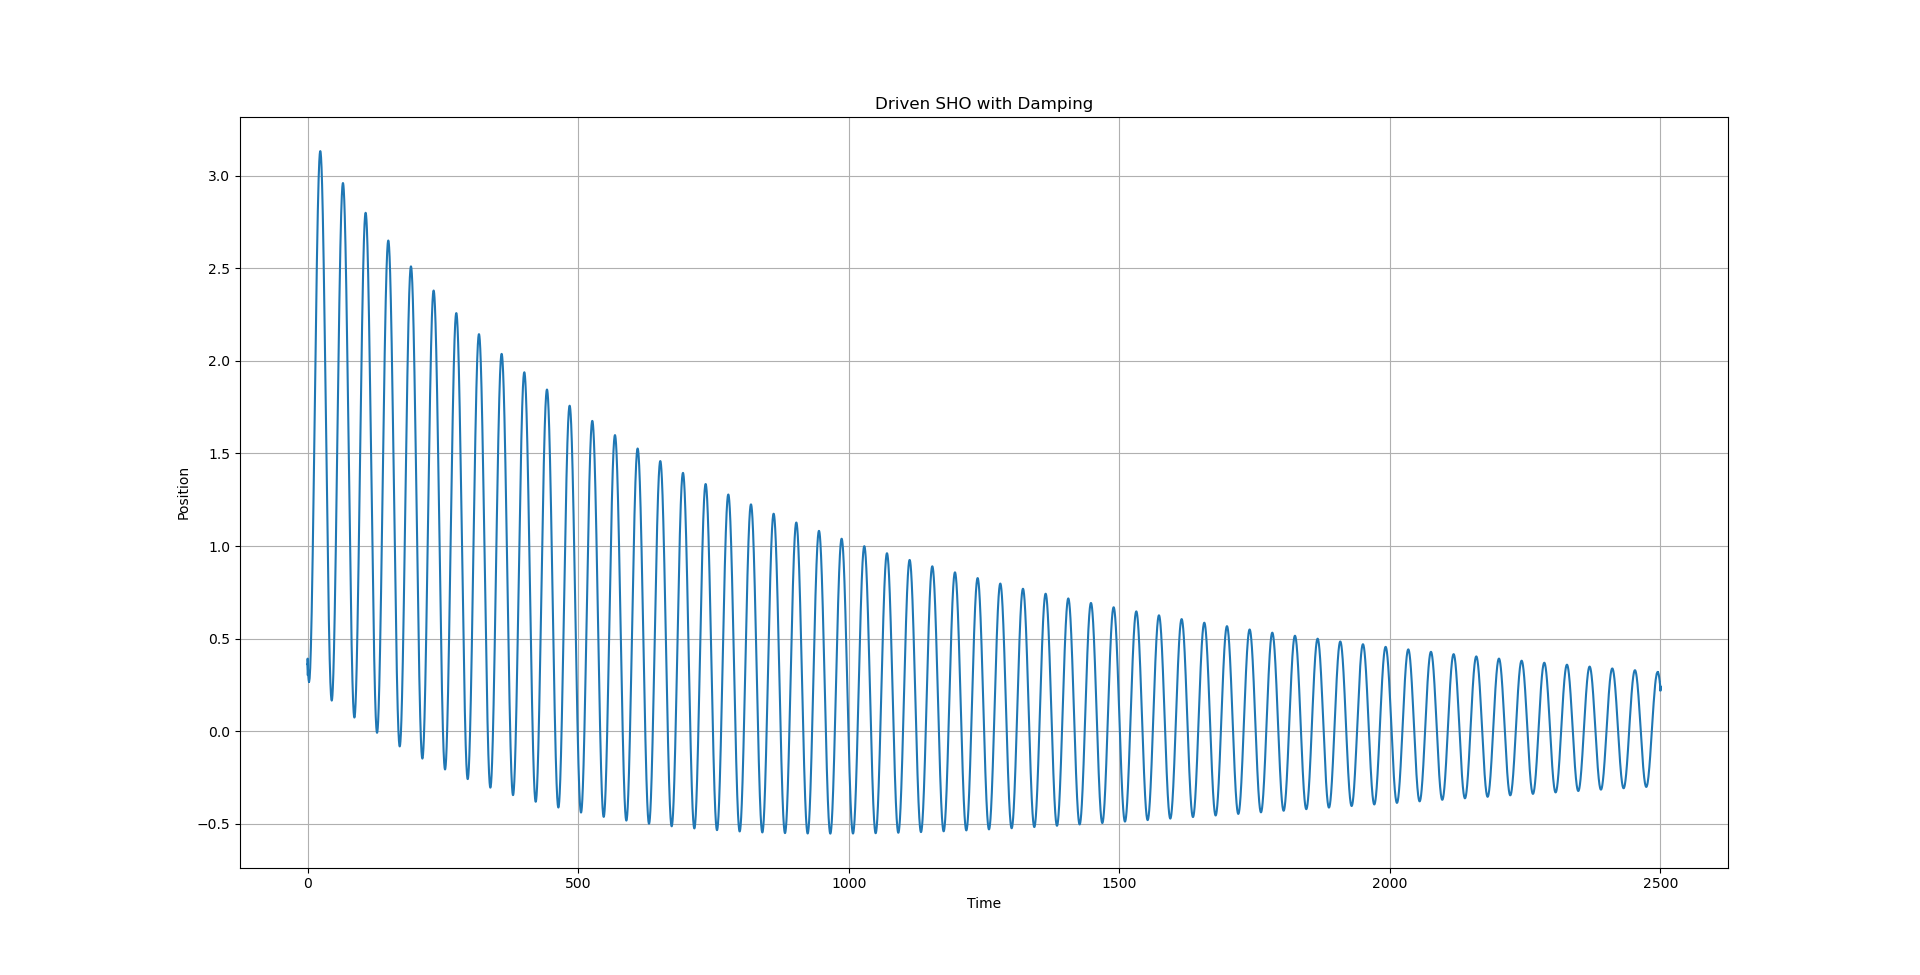
\includegraphics[width=100mm,height=\textheight,keepaspectratio]{images/driven_sho_equation_numerical.png}
    \caption{Defining \cref{eq:driven_sho_equation_initial_condition} as the initial condition, above is the solution to the driven SHO equation with damping using the FFT and IFFT algorithms in Python.}
    \label{fig:driven_sho_equation_numerical}
\end{figure}
%%%%%%%%%%%%%%%%%%%%%%%%%%%%%%%%%%%%%%%%%%%%%%%%%%%%%%%%%%%%%%%%%%%%%%%%%%%%%%%%%%%%%%%%%%

% \subsection{Competitive Lotka-Volterra Equations}
The Lotka-Volterra Equations (\cref{eq:lotka_volterra_1,eq:lotka_volterra_2}) were introduced earlier in \cref{section:background}. However, rather than being a predator-prey relationship, the competitive Lotka-Volterra Equations describes the relationship between two species competing over common resources. Furthermore, this competition leads to the logistic reproduction of the species which is more realistic than the exponential reproduction of the non-competitive model.

\subsubsection{Definition}
\noindent
Let us define an ecosystem with the following assumptions:
\begin{itemize}
    \item The population of the two species is described by the functions \(x(t)\) and \(y(t)\).
    \item The per capita growth rate of the populations are \(r_x\) and \(r_y\) respectively.
    \item The negative impact of population \(x\) due to population \(y\) is given by \(\alpha_{xy}\). Similarly, the negative impact of population \(y\) due to population \(x\) is given by \(\alpha_{yx}\).
    \item Due to seasons and other natural disasters, there will be a natural increase and decrease in resources. Thus, the carrying capacity \(K(t)\) for populations \(x\) and \(y\) will fluctuate.
\end{itemize}

\noindent
Thus, the competitive Lotka-Volterra equations for two species are defined as follows:
\begin{align}  
    \frac{dx}{dt} &= r_x x \left(1 - \left(\frac{x + \alpha_{xy} y}{K(t)}\right)\right) \label{eq:competitive_lv_1} \\ 
    \frac{dy}{dt} &= r_y y \left(1 - \left(\frac{y + \alpha_{yx} x}{K(t)}\right)\right) \label{eq:competitive_lv_2}
\end{align}

\subsubsection{Application of the Fourier Transform}
Let us take the Fourier Transform of \cref{eq:competitive_lv_1,eq:competitive_lv_2} with respect to \(t\). Thus, let \(X(\omega)\), \(Y(\omega)\), and \(K_hat(\omega)\) be the respective Fourier Transforms of \(x(t)\), \(y(t)\), and \(K(t)\) with respect to \(t\).

\begin{equation}
    \mathcal{F}_t \left\{ \frac{dx}{dt} \right\} = \mathcal{F}_t \left\{ r_x x \left(1 - \left(\frac{x + \alpha_{xy} y}{K(t)}\right)\right) \right\}
\end{equation}

\noindent
Using \cref{fourier_derivative},
\begin{align}
    \mathcal{F}_t \left\{ \frac{dx}{dt} \right\} &= i \omega \mathcal{F}_t \left\{ x(t) \right\} \\
    &= i \omega X(\omega)
\end{align}

\noindent
Using \cref{fourier_multiplication},
\begin{align}
    i \omega X(\omega) &= \frac{r_x}{2 \pi} \left( \mathcal{F}_t \left\{ x(t) \right\} * \mathcal{F}_t \left\{ 1 - \left(\frac{x + \alpha_{xy} y}{K(t)}\right) \right\} \right) \\
    &= \frac{r_x}{2 \pi} \left( X(\omega) * \mathcal{F}_t \left\{ 1 - \left(\frac{x + \alpha_{xy} y}{K(t)}\right) \right\} \right)
\end{align}

\noindent
Using \cref{fourier_linearity},
\begin{align}
    i \omega X(\omega) &= \frac{r_x}{2 \pi} \left( X(\omega) * \left( \mathcal{F}_t \left\{ 1 \right\} -  \mathcal{F}_t \left\{ \left(x + \alpha_{xy} y\right) \left( \frac{1}{K(t)} \right) \right\} \right) \right)
\end{align}

\noindent
Using \cref{fourier_multiplication} and \cref{fourier_linearity} again,
\begin{align}
    i \omega X(\omega) &= \frac{r_x}{2 \pi} \left( X(\omega) * \left( \mathcal{F}_t \left\{ 1 \right\} - \frac{1}{2 \pi} \left( \mathcal{F}_t \left\{ x + \alpha_{xy} y \right\} * \mathcal{F}_t \left\{ \frac{1}{K(t)} \right\} \right) \right) \right) \\
    i \omega X(\omega) &= \frac{r_x}{2 \pi} \left( X(\omega) * \left( \mathcal{F}_t \left\{ 1 \right\} - \frac{1}{2 \pi}  \left( \left( \mathcal{F}_t \left\{ x \right\} + \alpha_{xy} \mathcal{F}_t \left\{ y \right\} \right) * \mathcal{F}_t \left\{ \frac{1}{K(t)} \right\} \right) \right) \right) \\
    i \omega X(\omega) &= \frac{r_x}{2 \pi} \left( X(\omega) * \left( \mathcal{F}_t \left\{ 1 \right\} - \frac{1}{2 \pi}  \left( \left( X(\omega) + \alpha_{xy} Y(\omega) \right) * \mathcal{F}_t \left\{ \frac{1}{K(t)} \right\} \right) \right) \right)
\end{align}

\noindent
Following the same procedure for the \cref{eq:competitive_lv_2},

\subsubsection{Initial and Boundary Conditions}

\subsubsection{Numerical Solution to Competitive Lotka-Volterra Equation}
%%%%%%%%%%%%%%%%%%%%%%%%%%%%%%%%%%%%%%%%%%%%%%%%%%%%%%%%%%%%%%%%%%%%%%%%%%%%%%%%%%%%%%%%%%

% PDE to ODE Examples
\section{PDE to ODE Reduction}
Furthermore, the Fourier Transform serves as a powerful mathematical tool to solve partial differential equations (PDEs) by enabling the reduction of complex PDE systems to simpler ordinary differential equations (ODEs). Consequently, the system's complexity diminishes, paving the way for more manageable ODEs. This reduction not only facilitates the exploration of analytical solutions but also enhances the feasibility of employing numerical techniques like Euler's Method or Runge-Kutta methods for efficient computation. The utilization of Fourier Transform in this context offers a valuable approach to gaining deeper insights into the behavior and dynamics of various systems, making it a fundamental tool in the study of differential equations as shown by the following examples \citep{danchin2005fourier}.

\subsection{The Heat Equation}
Fourier Analysis was first discovered when Joseph Fourier first developed the Heat Equation. The Heat Equation models the flow of heat along a certain heat profile over time. In this example, a 1D solution will be derived and solved.

\subsubsection{Brief Derivation}
\noindent
Let us define a rod with the following assumptions:
\begin{itemize}
    \item The rod is of length \(L\) and is composed of an homogenous material with a heat diffusion coefficient \( \alpha^2 \).
    \item The rod is perfectly insulated along the Y and Z axes. Thus, heat can only flow along the X axis of the rod.
    \item The rod is thin enough such that the temperature of the rod at any cross-section is uniform.
    \item The rod is initially at a uniform temperature \(u(x,0) = f(x)\). Thus, the rod temperature at position \(x\) at time \(t\) is \(u(x,t)\).
\end{itemize}

% TODO: Is it worth it to actually derive the heat equation? It is beyond the scope of this paper.

\noindent
Thus, the heat equation in one dimension is defined as follows:
\begin{equation} \label{eq:heat_equation}
    \frac{\partial u}{\partial t} = \alpha^2 \nabla^2 u = \alpha^2 \frac{\partial^2 u}{\partial x^2}
\end{equation}

\noindent
Or in subscript notation,
\begin{equation} \label{eq:heat_equation_subscript}
    u_t = \alpha^2 u_{xx}
\end{equation}

\subsubsection{Application of the Fourier Transform}
Since \(u(x,t)\) is defined as the temperature of the rod at position \(x\) and time \(t\), we can apply the Fourier Transform to \(u(x,t)\) with respect to position \(x\) to reduce the PDE derived in the previous section into an ODE. Thus, let \(\hat{u}(\kappa,t)\) be the Fourier Transform of \(u(x,t)\) with respect to \(x\).
\begin{equation}
    \mathcal{F} \left\{ u_t \right\} = \mathcal{F} \left\{ \alpha^2 u_{xx} \right\}
\end{equation}

Using \cref{fourier_scaling},
\begin{equation}
    \mathcal{F} \left\{ u_t \right\} = \alpha^2 \mathcal{F} \left\{ u_{xx} \right\}
\end{equation}

Using \cref{fourier_derivative},
    \begin{align}
        \mathcal{F}\{ \frac{\partial^2 u(x, t)}{\partial x^2} \} & = i \kappa \mathcal{F}\{ \frac{d u(x, t)}{dx} \} \\
        & = -\kappa^2 \mathcal{F}\{ u(x, t) \} \\
        & = -\kappa^2 \hat{u}
    \end{align}

Therefore,
\begin{align}
    \mathcal{F} \left\{ u_t \right\} &= -\alpha^2 \kappa^2 \hat{u} \\
    \frac{d \hat{u}}{dt} &= -\alpha^2 \kappa^2 \hat{u} \label{eq:heat_equation_fourier}
\end{align}

\subsubsection{Numerical Solution to Heat Equation} % TODO: Link the Python code for this numerical integration in the appendix.
\cref{eq:heat_equation_fourier} is a decoupled ODE that can be easily numerically integrated. A numerical solution to \cref{eq:heat_equation_fourier} using a fifth-order Runge-Kutta approximation in Python is presented below:

\begin{figure}[H]
    \centering
    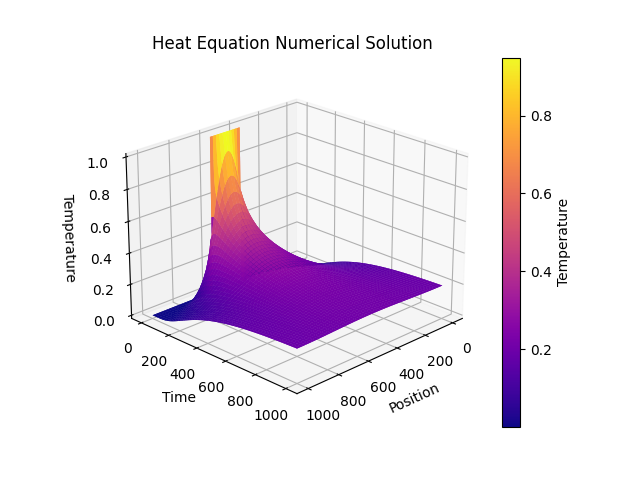
\includegraphics[width=110mm,height=\textheight,keepaspectratio]{images/heat_equation_numerical.png}
    \caption{Using a simple square waveform as the initial temperature function of the rod, this plot shows the temperature change along \(x\) and \(t\) by performing a numerical integration of \cref{eq:heat_equation_fourier}.}
    \label{fig:heat_equation_numerical}
\end{figure}

% \subsubsection{Analytical Solution to Heat Equation} 
% This is a maybe section. Possibly replace this section with a section on the applicability of the Fourier Transform to reduce PDEs to ODEs...?
%%%%%%%%%%%%%%%%%%%%%%%%%%%%%%%%%%%%%%%%%%%%%%%%%%%%%%%%%%%%%%%%%%%%%%%%%%%%%%%%%%%%%%%%%%

\subsection{The Wave Equation}

\subsubsection{Brief Derivation}

\subsubsection{Application of the Fourier Transform}

\subsubsection{Numerical Solution to Wave Equation}

% \subsubsection{Analytical Solution to Wave Equation} 
% This is a maybe section. Possibly replace this section with a section on the applicability of the Fourier Transform to reduce PDEs to ODEs...?
%%%%%%%%%%%%%%%%%%%%%%%%%%%%%%%%%%%%%%%%%%%%%%%%%%%%%%%%%%%%%%%%%%%%%%%%%%%%%%%%%%%%%%%%%%

\subsection{Black-Scholes Equation}
The Black-Scholes equation is a PDE that describes the depreciation in the price of a European call or put option at a given stock price and a given time.

\subsubsection{Definition}
\noindent
Let us define a European call or put option with the following assumptions:
\begin{itemize}
    \item Define \(\sigma\) to be the volatility of the underlying asset and \(r\) be the risk-free interest rate.
    \item The initial valuation of an option at a fixed stock price is  \(V(S,0) = f(t)\). Thus, the option at a given underlying stock price \(S\) and a given option expiry time \(t\) is \(V(S,t)\).
\end{itemize}

\noindent
Thus, the Black-Scholes equation is defined as follows \citep{Buchanan_black_scholes_2014}:
\begin{equation} \label{eq:black_scholes_equation}
    \frac{\partial V}{\partial t} + \frac{1}{2}\sigma^2 S^2 \frac{\partial^2 V}{\partial S^2} + rS\frac{\partial V}{\partial S} - rV = 0
\end{equation}

\subsubsection{Application of the Fourier Transform}
Let us take the Fourier Transform of \cref{eq:black_scholes_equation} with respect to \(S\). Thus, let \(\hat{V}(\kappa, t)\) be the Fourier Transform of \(V(S, t)\) with respect to \(S\).

\begin{equation}
    \mathcal{F}_S \left\{ \frac{\partial V}{\partial t} + \frac{1}{2}\sigma^2 S^2 \frac{\partial^2 V}{\partial S^2} + rS\frac{\partial V}{\partial S} -  rV \right\} = \mathcal{F}_S \left\{ 0 \right\}
\end{equation}

\noindent
Using \cref{fourier_linearity} and the fact that the integral of the zero function is zero,
\begin{equation}
    \mathcal{F}_S \left\{ \frac{\partial V}{\partial t} \right\} + \mathcal{F}_S \left\{ \frac{1}{2}\sigma^2 S^2 \frac{\partial^2 V}{\partial S^2} \right\} + \mathcal{F}_S \left\{ rS\frac{\partial V}{\partial S} \right\} - \mathcal{F}_S \left\{ rV \right\} = 0
\end{equation}

\noindent
Using \cref{fourier_scaling},
\begin{equation} 
    \mathcal{F}_S \left\{ \frac{\partial V}{\partial t} \right\} + \frac{1}{2}\sigma^2 \mathcal{F}_S \left\{ S^2 \frac{\partial^2 V}{\partial S^2} \right\} + r \mathcal{F}_S \left\{ S\frac{\partial V}{\partial S} \right\} - r \mathcal{F}_S \left\{ V \right\} = 0
\end{equation}

\noindent
Using \cref{fourier_derivative},
\begin{align}
    \mathcal{F}_S \left\{ \frac{\partial V}{\partial S} \right\} &= i \kappa \mathcal{F}_S \left\{ V(S, t) \right\} \\
    &= i \kappa \hat{V}(\kappa, t) \\
    \mathcal{F}_S \left\{ \frac{\partial^2 V}{\partial S^2} \right\} & = i \kappa \mathcal{F}_S \left\{ \frac{\partial V}{\partial S} \right\} \\
    & = -\kappa^2 \hat{V}(\kappa, t)
\end{align}

\noindent
Using \cref{fourier_multiplication},
\begin{align}
    \mathcal{F}_S \left\{ S\frac{\partial V}{\partial S} \right\} &= \frac{1}{2 \pi}( \mathcal{F}_S \left\{ S \right\} * \mathcal{F}_S \left\{ \frac{\partial V}{\partial S} \right\} ) \\
    &= \frac{1}{2 \pi}( \mathcal{F}_S \left\{ S \right\} * i \kappa \hat{V} ) \\
    \mathcal{F}_S \left\{ S^2 \frac{\partial^2 V}{\partial S^2} \right\} &= \frac{1}{2 \pi}( \mathcal{F}_S \left\{ S^2 \right\} * \mathcal{F}_S \left\{ \frac{\partial^2 V}{\partial S^2} \right\} ) \\
    &= \frac{1}{2 \pi}( \mathcal{F}_S \left\{ S^2 \right\} * -\kappa^2 \hat{V} ) \\
\end{align}

\noindent
Therefore,
\begin{align}
    \frac{\partial \hat{V}}{\partial t} + \frac{1}{2}\sigma^2 \mathcal{F}_S \left\{ S^2 \frac{\partial^2 V}{\partial S^2} \right\} + r \mathcal{F}_S \left\{ S\frac{\partial V}{\partial S} \right\} - r \hat{V} &= 0 \\
    \frac{\partial \hat{V}}{\partial t} + \frac{1}{2}\sigma^2 \frac{1}{2 \pi}( \mathcal{F}_S \left\{ S^2 \right\} * -\kappa^2 \hat{V} ) + r \frac{1}{2 \pi}( \mathcal{F}_S \left\{ S \right\} * i \kappa \hat{V} ) - r \hat{V} &= 0 \\
    \frac{\partial \hat{V}}{\partial t} - \frac{1}{4 \pi}\sigma^2 \kappa^2 ( \mathcal{F}_S \left\{ S^2 \right\} * \hat{V} ) + \frac{1}{2 \pi} r i \kappa ( \mathcal{F}_S \left\{ S \right\} * \hat{V} ) - r \hat{V} &= 0
\end{align}

\noindent
Thus,
\begin{equation}
    \label{eq:black_scholes_fourier}
    \frac{d \hat{V}}{dt} = \frac{1}{4 \pi}\sigma^2 \kappa^2 ( \mathcal{F}_S \left\{ S^2 \right\} * \hat{V} ) - \frac{1}{2 \pi} r i \kappa ( \mathcal{F}_S \left\{ S \right\} * \hat{V} ) + r \hat{V}
\end{equation}

\subsubsection{Initial and Boundary Conditions}
A simple linear function will be used as the initial option price for the ODE:
\begin{align}
    V(S_{max}, t)=0.15t + 148.5 \label{eq:black_scholes_equation_initial_condition}
\end{align}

\noindent
If the underlying stock of an option is worth nothing, then the option itself is worth nothing. This boundary condition can expressed as follows:
\begin{align}
    V(0, t) = 0
\end{align}

\noindent
Furthermore, since a call option is advantageous when the stock price \(S\) is greater than the exercise price \(E\) and a put option is only advantageous when the exercise price \(E\) is greater than the stock price \(S\), the following boundary conditions must be true.
\begin{align}
    V(S, t) = 
    \begin{cases}
        max(S-E, 0) & \text{if call option} \\
        max(E-S, 0) & \text{if put option}
    \end{cases}
\end{align}

\subsubsection{Numerical Solution to Black-Scholes Equation}
\cref{eq:black_scholes_equation} is a first-order ODE that can be easily numerically integrated. A numerical solution to \cref{eq:black_scholes_fourier} using a fifth-order Runge-Kutta approximation in Python is presented below. The Python code can be found in \cref{code:black_scholes_equation}.

\begin{figure}[H]
    \centering
    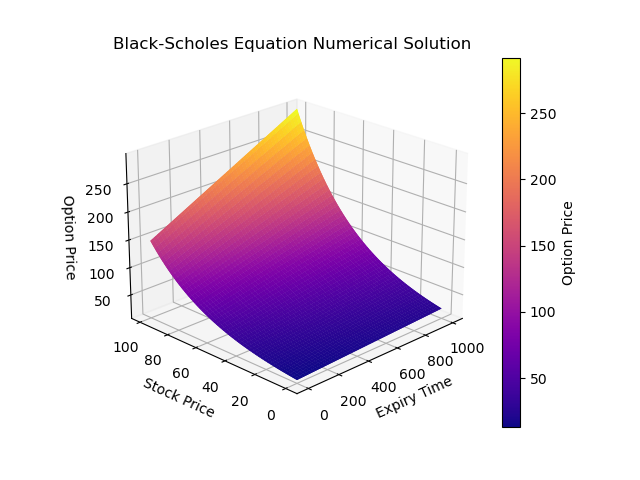
\includegraphics[width=100mm,height=\textheight,keepaspectratio]{images/black_scholes_equation_numerical.png}
    \caption{Defining the initial option price as \cref{eq:black_scholes_equation_initial_condition}, this plot shows the temperature change along \(S\) and \(t\) by performing a numerical integration of \cref{eq:black_scholes_fourier}.}
    \label{fig:black_scholes_equation_numerical}
\end{figure}
%%%%%%%%%%%%%%%%%%%%%%%%%%%%%%%%%%%%%%%%%%%%%%%%%%%%%%%%%%%%%%%%%%%%%%%%%%%%%%%%%%%%%%%%%%

% Strengths and Limitations of the Fourier Transform
\section{Limitations of Fourier Analysis}
As shown by the various examples, Fourier transforms are a powerful tool for solving differential equations. However, there are certain situations where Fourier transforms may not be applicable or effective. Here are a few cases \citep{howell2016principles}:

% TODO: Rephrase and Adjust as needed...
% TODO: Make sure the conclusion and the limitations talk about similar things for continuity.
\begin{enumerate}
    % Talk about how important linearity is as a concept in solving differential equations. How this is important for Fourier Transforms.
    \item Nonlinear Equations: Fourier transforms are generally not applicable to nonlinear differential equations. The transforms rely on linearity properties, such as superposition and scaling, which do not hold for nonlinear equations. In such cases, other techniques like numerical methods or perturbation methods may be more suitable.
    \item Variable Coefficients: Fourier transforms are most commonly used for differential equations with constant coefficients. When the coefficients of the differential equation are functions of the independent variable or have a complicated dependence, the application of Fourier transforms becomes more challenging. In such cases, specialized techniques like Laplace transforms or numerical methods may be employed.
    \item Finite Boundaries: Fourier transforms are well-suited for solving differential equations on unbounded domains or for periodic problems. However, when dealing with differential equations on finite intervals or with non-periodic boundary conditions, additional techniques like separation of variables, finite difference methods, or numerical techniques may be required.
    \item Discontinuous Functions: Fourier transforms rely on the assumption that the functions involved are well-behaved and continuous. If the functions or their derivatives exhibit discontinuities, the Fourier transform may not be directly applicable. Techniques like generalized functions (e.g., distributions) or other specialized methods may be employed in these cases.
    \item Stochastic or Random Processes: Fourier transforms are primarily used for deterministic differential equations. When dealing with stochastic or random processes, such as in the field of stochastic differential equations, other tools like stochastic calculus, probability theory, or numerical simulation methods may be more appropriate.
\end{enumerate}
%%%%%%%%%%%%%%%%%%%%%%%%%%%%%%%%%%%%%%%%%%%%%%%%%%%%%%%%%%%%%%%%%%%%%%%%%%%%%%%%%%%%%%%%%%